\setcounter{chapter}{3}
\chapter{Conclusion and Future Work}\label{sec:conclusionfuturework}
In this chapter, we describe the phases of our plan for exploring
the research challenges and investigating the research issues
identified in Chapter 3. This chapter also includes research
methodology and future publication plan.

\section {Conclusion}

In this report, we presented research problems and questions we
aim to address in the thesis and proposed some preliminary results
about a cooperative game theory-based model for the aggregation of
web services within communities. The goal of our services is to
maximize efficiency by collaborating and forming stable
coalitions. Our method considers stability and fairness for all
web services within a community and offers an applicable mechanism
for membership requests and selection of web services. The
ultimate goal is to increase revenue by improving user
satisfaction, which comes from the ability to perform more tasks
with high quality. Simulation results show that our approximation
algorithms are polynomial in complexity and provide web services
and community owners with applicable and near-optimal decision
making mechanisms.

%As future work, we would like to perform more analytical and
%theoretical analysis on the convexity condition and also minimal $\epsilon$ values in \emph{$\epsilon$-core} solution concepts based on the
%characteristic function in web service applications. From web service perspective, the
%work can be extended to consider web service compositions where a
%group of web services having different set of skills cooperate to
%perform composite tasks. Also bargaining theory from cooperating
%game theory concepts can be used to help web services resolve the
%instability and unfairness issues by side payments.

\section {Future Plan and Timeline}

\indent The future goals in this Ph.D. research work are:

\begin{itemize}
\item Analyzing other cooperative solution concepts such as Kernel
and Nucleolus where payoff division is guaranteed to exist and may
have optimal results.

\item Applying other valuation function in our scenarios using for
instance Weighted Voting Games (WCG) in order to develop a
multiple weighted algorithm to find best coalition structures
satisfying different weights on each community.

\item Analyzing the impact of Q-learning and reinforcement
learning on the performance of our model.

\item Developing an approximation algorithm for shapely value
payoff distribution vector in community setting.

\item Developing a community membership algorithm technique for
our agents in "incomplete information" settings.

%\item Developing an open source, Java based Tool, with UI for
%solving Core and Shapely solution concepts based on different
%input valuation functions.
\end{itemize}


    \begin{figure}
                \begin{center}
%                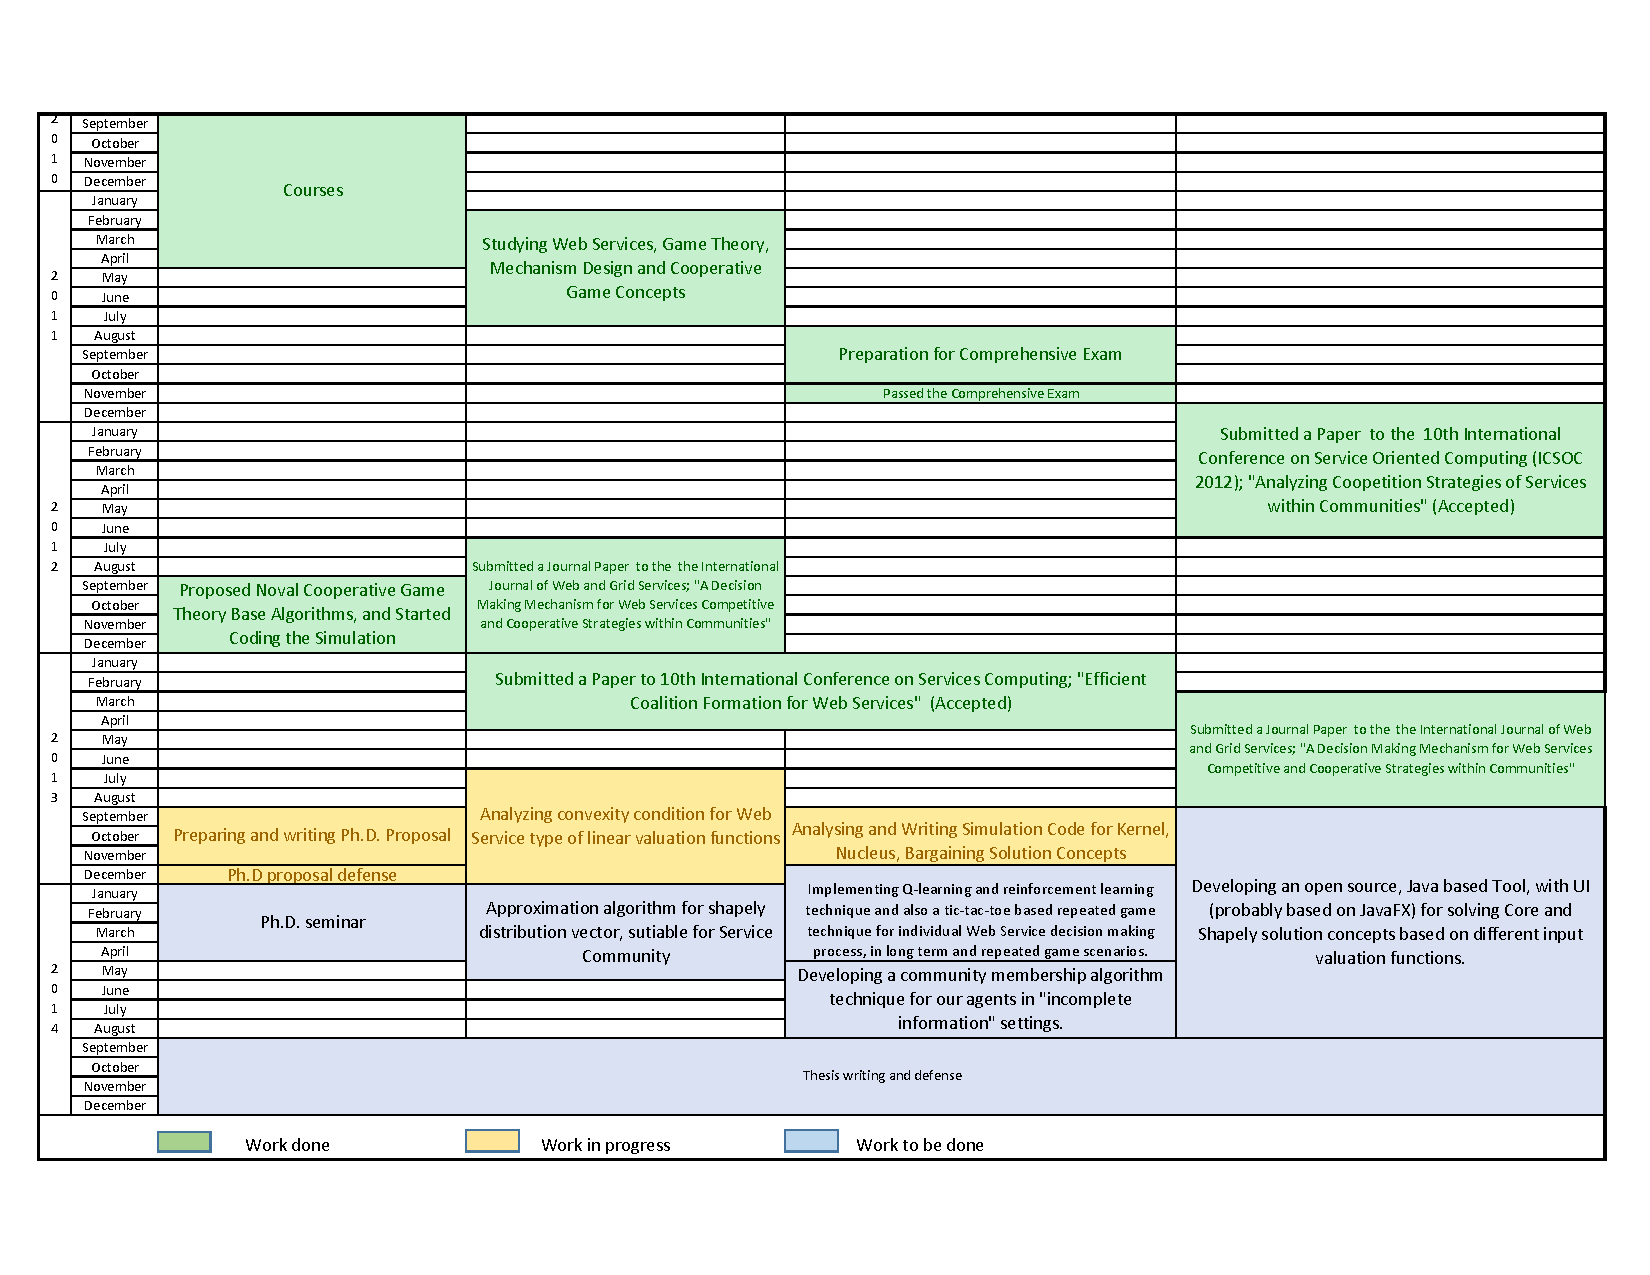
\includegraphics[width=16cm, height=22cm]{timeline/timetable.pdf}\label{Timetable}
                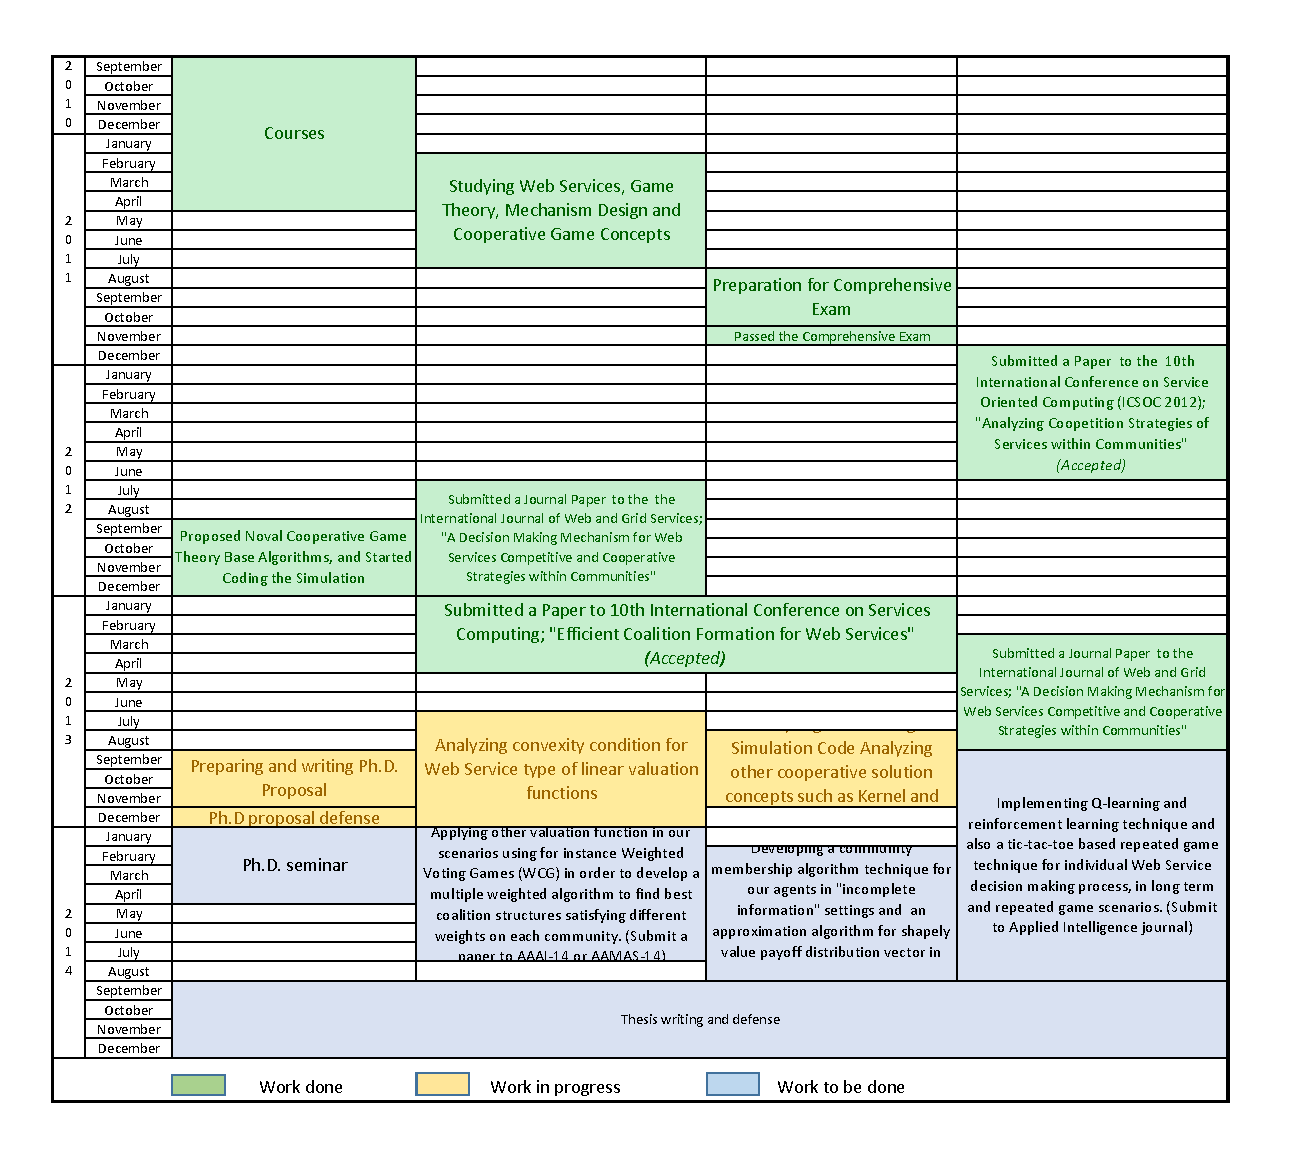
\includegraphics[width=16cm]{timeline/timetable1.eps}\label{Timetable}
                \caption{Research milestones and timeline}
                \end{center}
    \end{figure}
